\subsection{Dataset and Data Preprocessing}

\subsubsection{VisDrone Dataset}

The object detection model is trained and evaluated on the VisDrone2019-DET dataset, a large-scale benchmark designed for drone-based visual understanding tasks. The dataset contains aerial images captured by unmanned aerial vehicles (UAVs) under diverse urban scenarios, including streets, intersections, campuses, and pedestrian areas. Compared with conventional ground-view datasets, VisDrone presents additional challenges such as small object sizes, heavy occlusion, large scale variations, and dense object distributions.

The dataset provides annotated bounding boxes for multiple object categories, including pedestrians, cars, buses, bicycles, trucks, and so on. Representative samples from the dataset are shown in Figure~\ref{fig:visdrone_samples}. Both daytime and nighttime scenes contain dense object distributions with many small-scale targets, which makes the detection task considerably more challenging.

\begin{figure}[htbp]
    \centering
    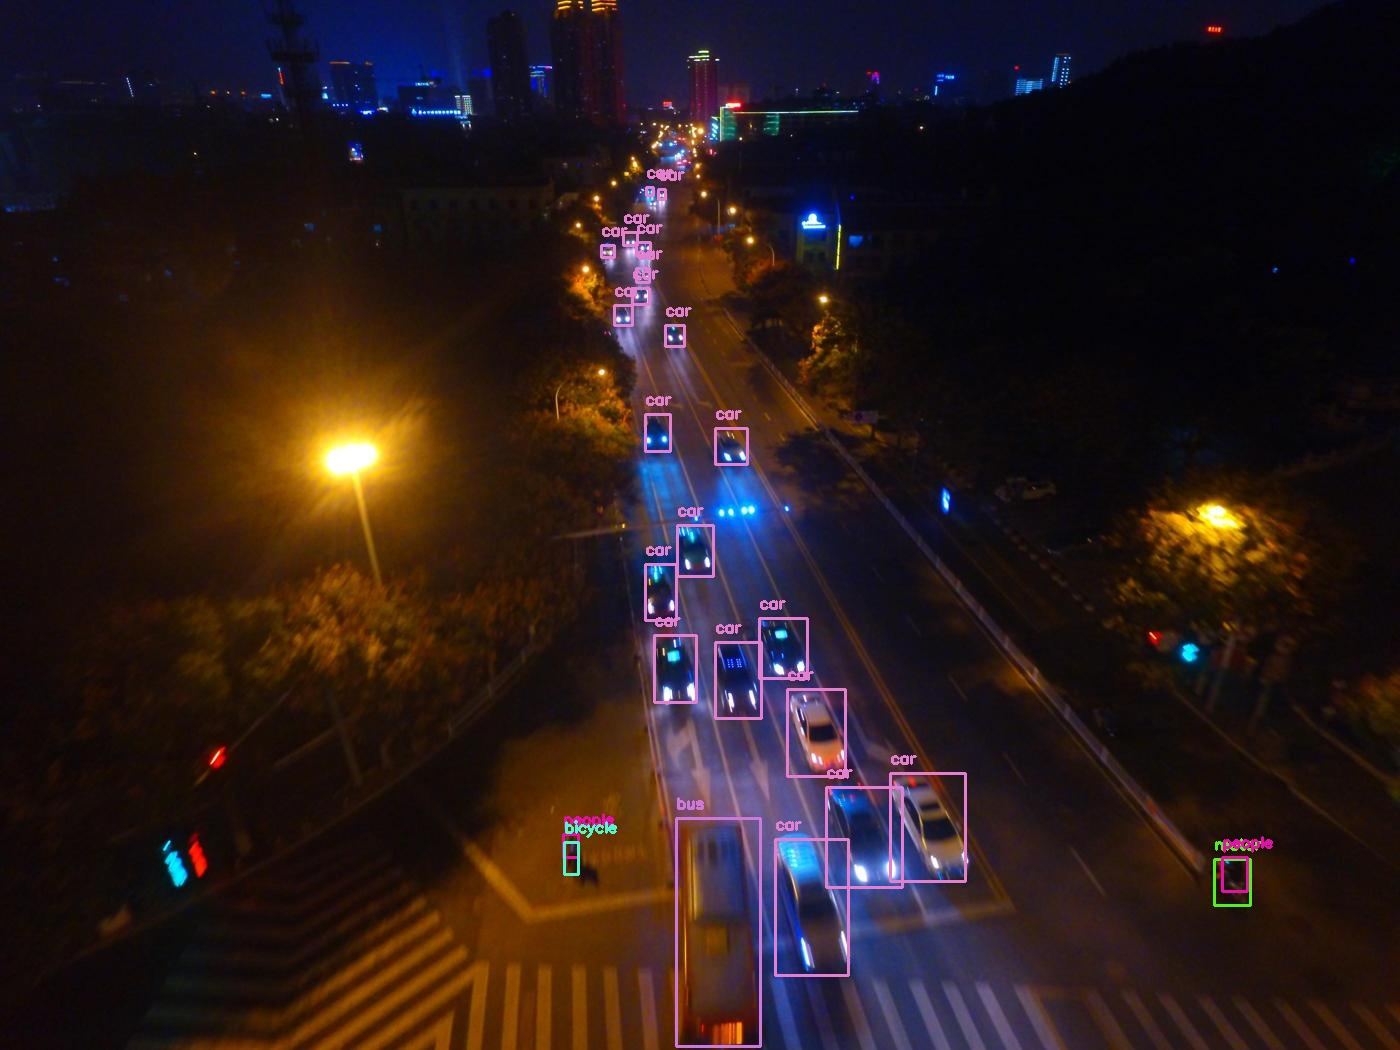
\includegraphics[width=0.48\textwidth]{figures/task2/data_visualization_9999950_00000_d_0000067.jpg}
    \hfill
    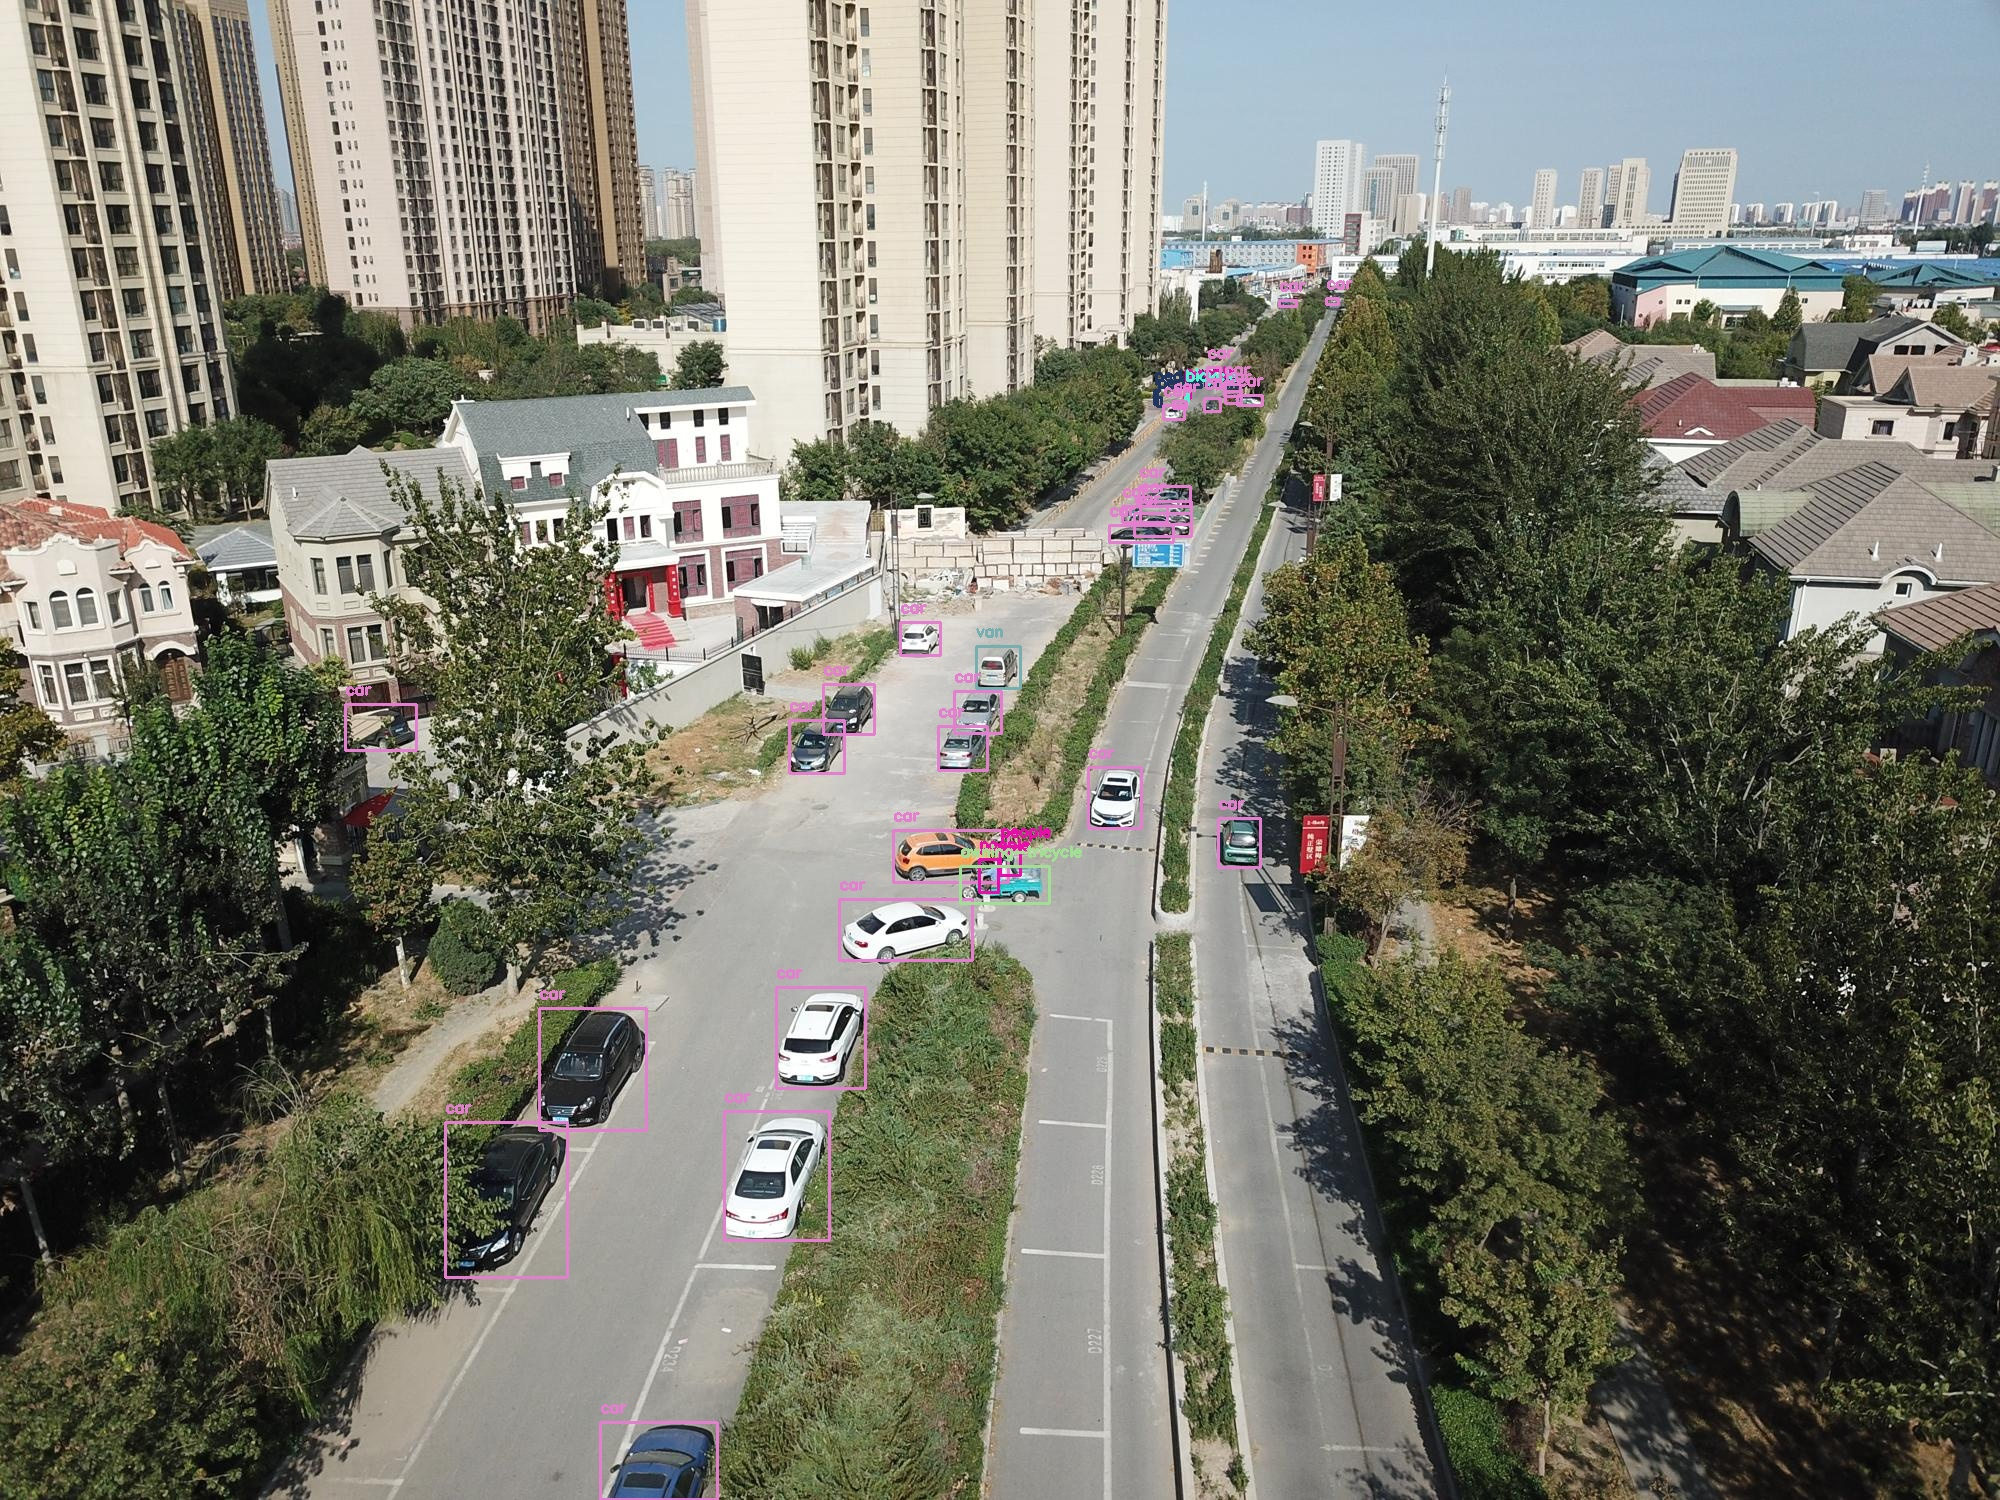
\includegraphics[width=0.48\textwidth]{figures/task2/data_visualization_9999998_00294_d_0000247.jpg}
    \caption{Representative samples from the VisDrone2019-DET dataset. The left image shows a nighttime scene, while the right image shows a daytime scene. Both scenes contain dense distributions of small objects.}
    \label{fig:visdrone_samples}
\end{figure}

\subsubsection{Data Preparation and Preprocessing}

The original VisDrone annotations use pixel-based bounding boxes represented as
\[
(L, T, w, h),
\]
where $(L, T)$ denotes the top-left coordinate of the bounding box, and $w$, $h$ denote the width and height of the bounding box in pixels.

For YOLO training, the annotations are converted into normalized center-coordinate format:
\[
(x_c, y_c, w_n, h_n),
\]
where
\[
x_c = \frac{L + \frac{w}{2}}{W}, \qquad
y_c = \frac{T + \frac{h}{2}}{H},
\]
\[
w_n = \frac{w}{W}, \qquad
h_n = \frac{h}{H}.
\]
Here, $W$ and $H$ denote the image width and height, respectively.

The processed dataset is reorganized into the standard YOLO directory structure with separate image and label folders for the training and validation splits. During preprocessing, category~0 (ignored regions) and category~11 (others) are removed to avoid ambiguous supervision signals during training.

In addition, Mosaic augmentation is enabled during training. Mosaic augmentation combines four training images into a single composite image, increasing object scale diversity and improving the robustness of the detector in dense aerial scenes with small objects and partial occlusions.
